\model{Hand of Cards}

Creating an array of objects is typically a 3-step process:

\begin{center}
\begin{minipage}[t]{155pt}

1. Declare the array \\[1ex]
\java{Card[] hand;}

\end{minipage}
\begin{minipage}[t]{155pt}

2. Instantiate the array \\[1ex]
\java{hand = new Card[5];}

\end{minipage}
\begin{minipage}[t]{155pt}

3. Instantiate each object \\[1ex]
\java{hand[0] = new Card(4, 2);}
\java{hand[1] = new Card(3, 1);}

\end{minipage}
\end{center}

\begin{center}
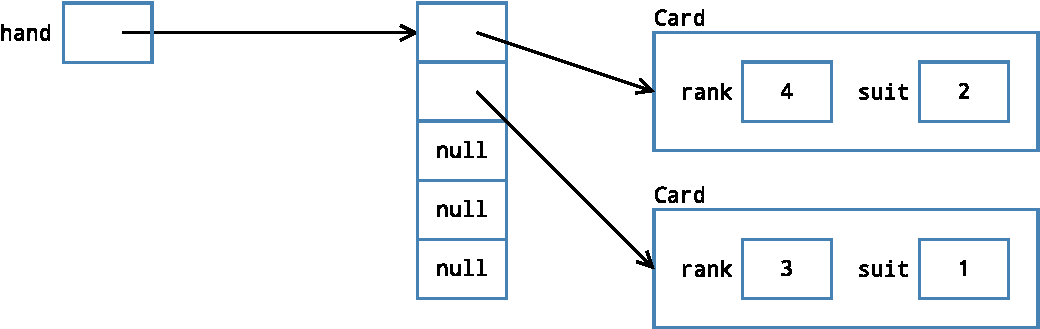
\includegraphics[width=465pt]{cards-array.pdf}
\end{center}


\quest{20 min}


\Q What is the type of the local variable \java{hand}?
What is the value of \java{hand} {\it before} step 2?
What is the value of \java{hand} {\it after} step 2?

\begin{answer}[3em]
The variable \java{hand} is an array of \java{Card} objects.
Before step 2, it's uninitialized (i.e., you can't read its value).
After step 2, its value is the memory location of the first array element.
\end{answer}


\Q When you create an array (e.g., ~\java{new Card[5]}) what is the initial value of each element?

\begin{answer}
The initial values are automatically set to null (for reference types). For arrays of integers, it's 0; for doubles, it's 0.0; for booleans, it's {\tt false}; for characters, it's the unicode character \chr{\textbackslash u0000}.
\end{answer}


\Q When you construct a new object (e.g., ~\java{new Card(4, 2)}) what are the initial values of its attributes (e.g., ~\java{this.rank})?

\begin{answer}
It depends on the constructor. For the \java{Card} class, the attributes \java{rank} and \java{suit} are initialized from the parameters. If there is no constructor, Java automatically initializes attributes to zero (or equivalent).
\end{answer}


\comment{The \java{new} operator finds a memory location to store an array or object.
Java automatically determines how much memory is needed and initializes the contents of the corresponding memory cells to zero.
That's why array elements and object attributes have default values, whereas local variables (not allocated with \java{new}) must be initialized before they are used.}


\Q \label{random}
Describe in your own words what the following code does.
Be sure to explain how the random part works.

\begin{quote}
\java{int index = (int) (Math.random() * hand.length);} \\
\java{hand[index] = null;}
\end{quote}

\begin{answer}
\java{Math.random()} returns a value in the range [0, 1).
Multiplying that value by \java{hand.length} and then casting it to an integer gives a value in the range 0..5 inclusive.
So this statement randomly sets one of the \java{Card} references to {\tt null}.
\end{answer}


\Q \label{forcard}
What is the result of running the loop below?
Explain why the if-statement is necessary.

\begin{javalst}
for (int i = 0; i < hand.length; i++) {
    if (hand[i] != null) {
        int suit = hand[i].getSuit();
        System.out.println("The suit of #" + i + " is " + Card.SUITS[suit]);
    }
}
\end{javalst}

\begin{answer}[3em]
The loop prints the suits of all cards in the hand.
Because some of the cards are {\tt null}, the if-statement prevents {\tt NullPointerException}.
\end{answer}


\Q The \emph{enhanced for loop} allows you to iterate the elements of an array.
Another name for this structure is the ``for each'' loop.
Rewrite the following example using a standard for loop.

\vspace{1ex}
\begin{javalst}
String[] days = {"Sun", "Mon", "Tue", "Wed", "Thu", "Fri", "Sat"};
for (String day : days) {
    System.out.println(day + " is a great day!");
}
\end{javalst}
\vspace{-1em}

\begin{answer}
\begin{javaans}
for (int i = 0; i < days.length; i++) {
    System.out.println(days[i] + " is a great day!");
}
\end{javaans}
\end{answer}


\Q In contrast to enhanced for loops, what does a standard for loop iterate?
Why would it be misleading to name the enhanced for loop variable \java{i} instead of \java{day}?

\begin{answer}[2em]
Standard for loops typically iterate indexes; that's why the variable is usually named \java{i}.
\end{answer}


\Q \label{foreach}
Rewrite the loop in \ref{forcard} using an enhanced for loop.
Use an appropriate variable name for the \java{Card} object (i.e., not \java{i}).
For simplicity, you may omit the \java{System.out.println} line.

\begin{answer}[6em]
\begin{javaans}
for (Card card : hand) {
    if (card != null) {
        int suit = card.getSuit();
    }
}
\end{javaans}
\end{answer}
